The HPS experiment data acquisition and trigger system handles the acquisition of data and 
distribution of triggers for three sub-detectors; the SVT, ECal and the muon detector. There 
are two front end electronic systems; the SVT is readout with 128-channel integrated circuits
 supported by Advanced Telecom Communications Architecture~\cite{atca} (ATCA) hardware
 while the ECal and muon detectors signals are processed by VXS based hardware. The 
 the Level 1 trigger receives input from the ECal and muon detectors only to form a decision 
 on which events to be read out.  The triggered events are acquired from the three subsystems and are processed in the data acquisition system outlined in 
 Fig.~\ref{fig:daq_hardware_overview}.
\begin{figure*}[t]
%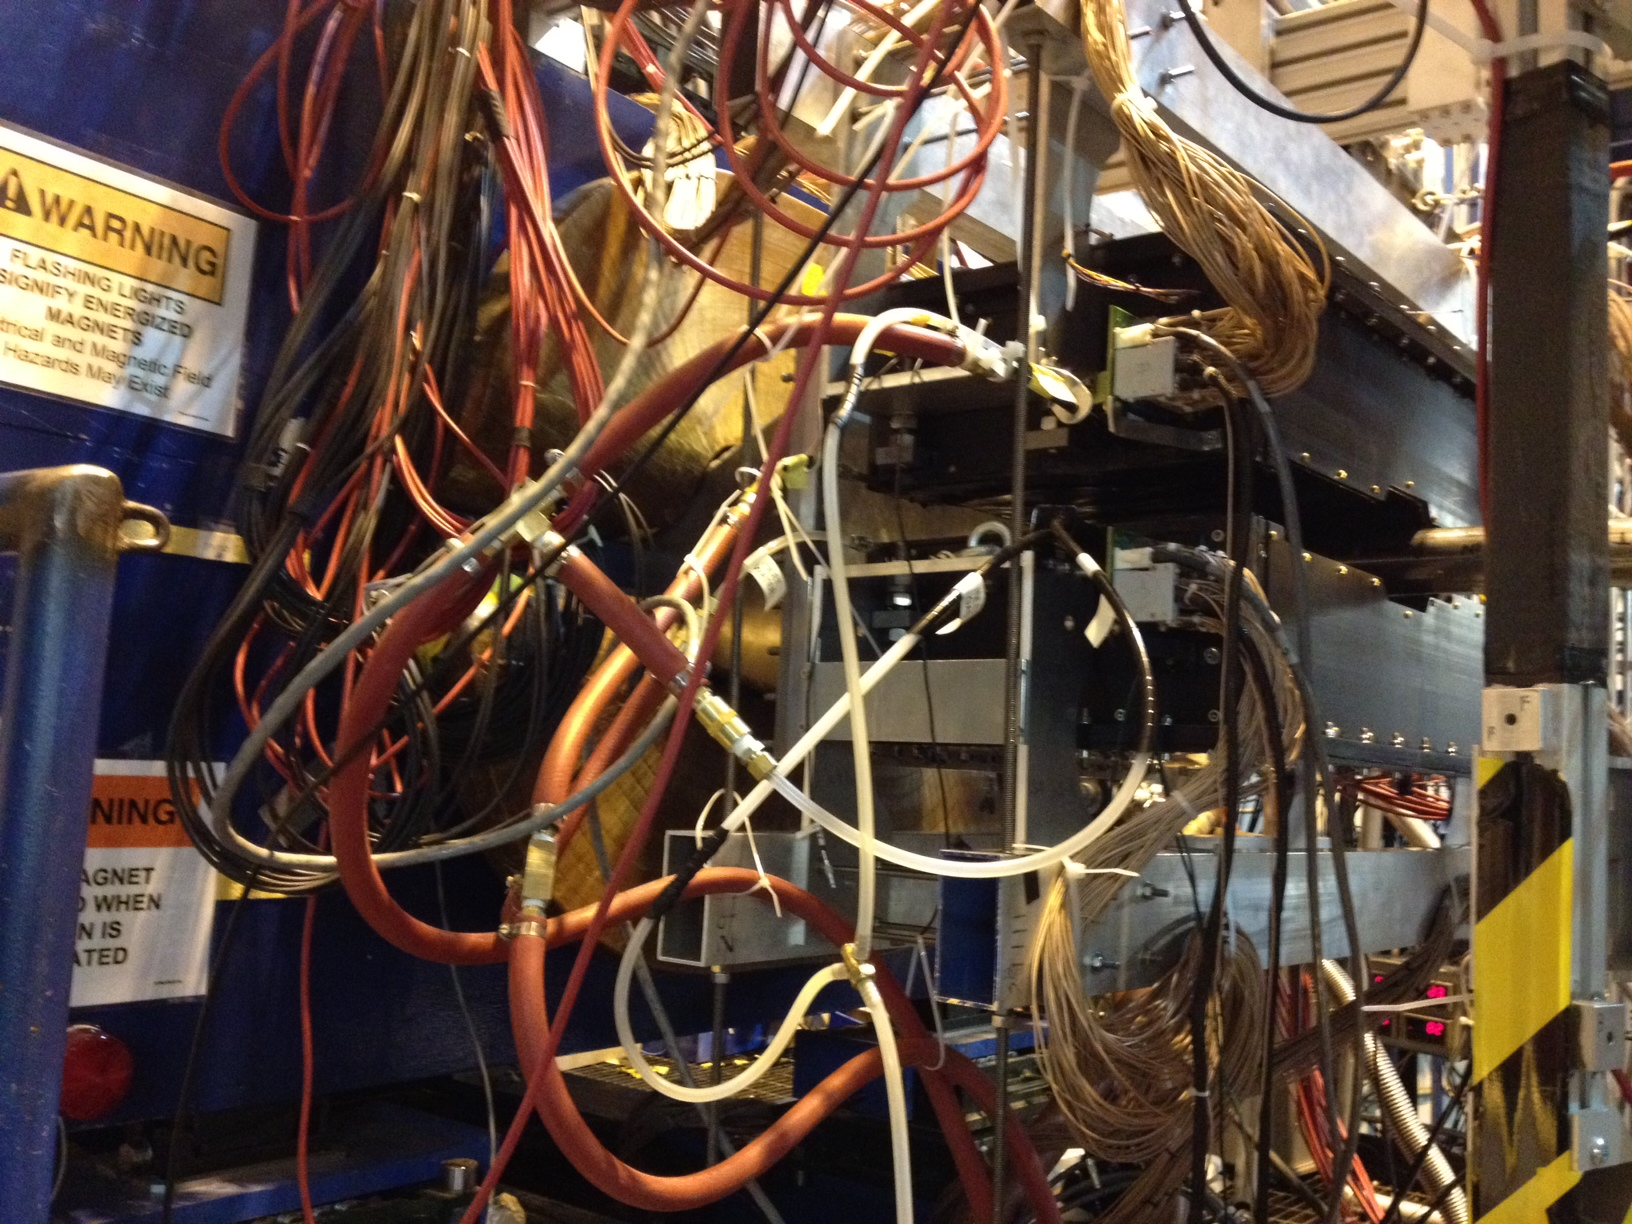
\includegraphics[ scale=0.25]{test2012/ecal_mounted.JPG}
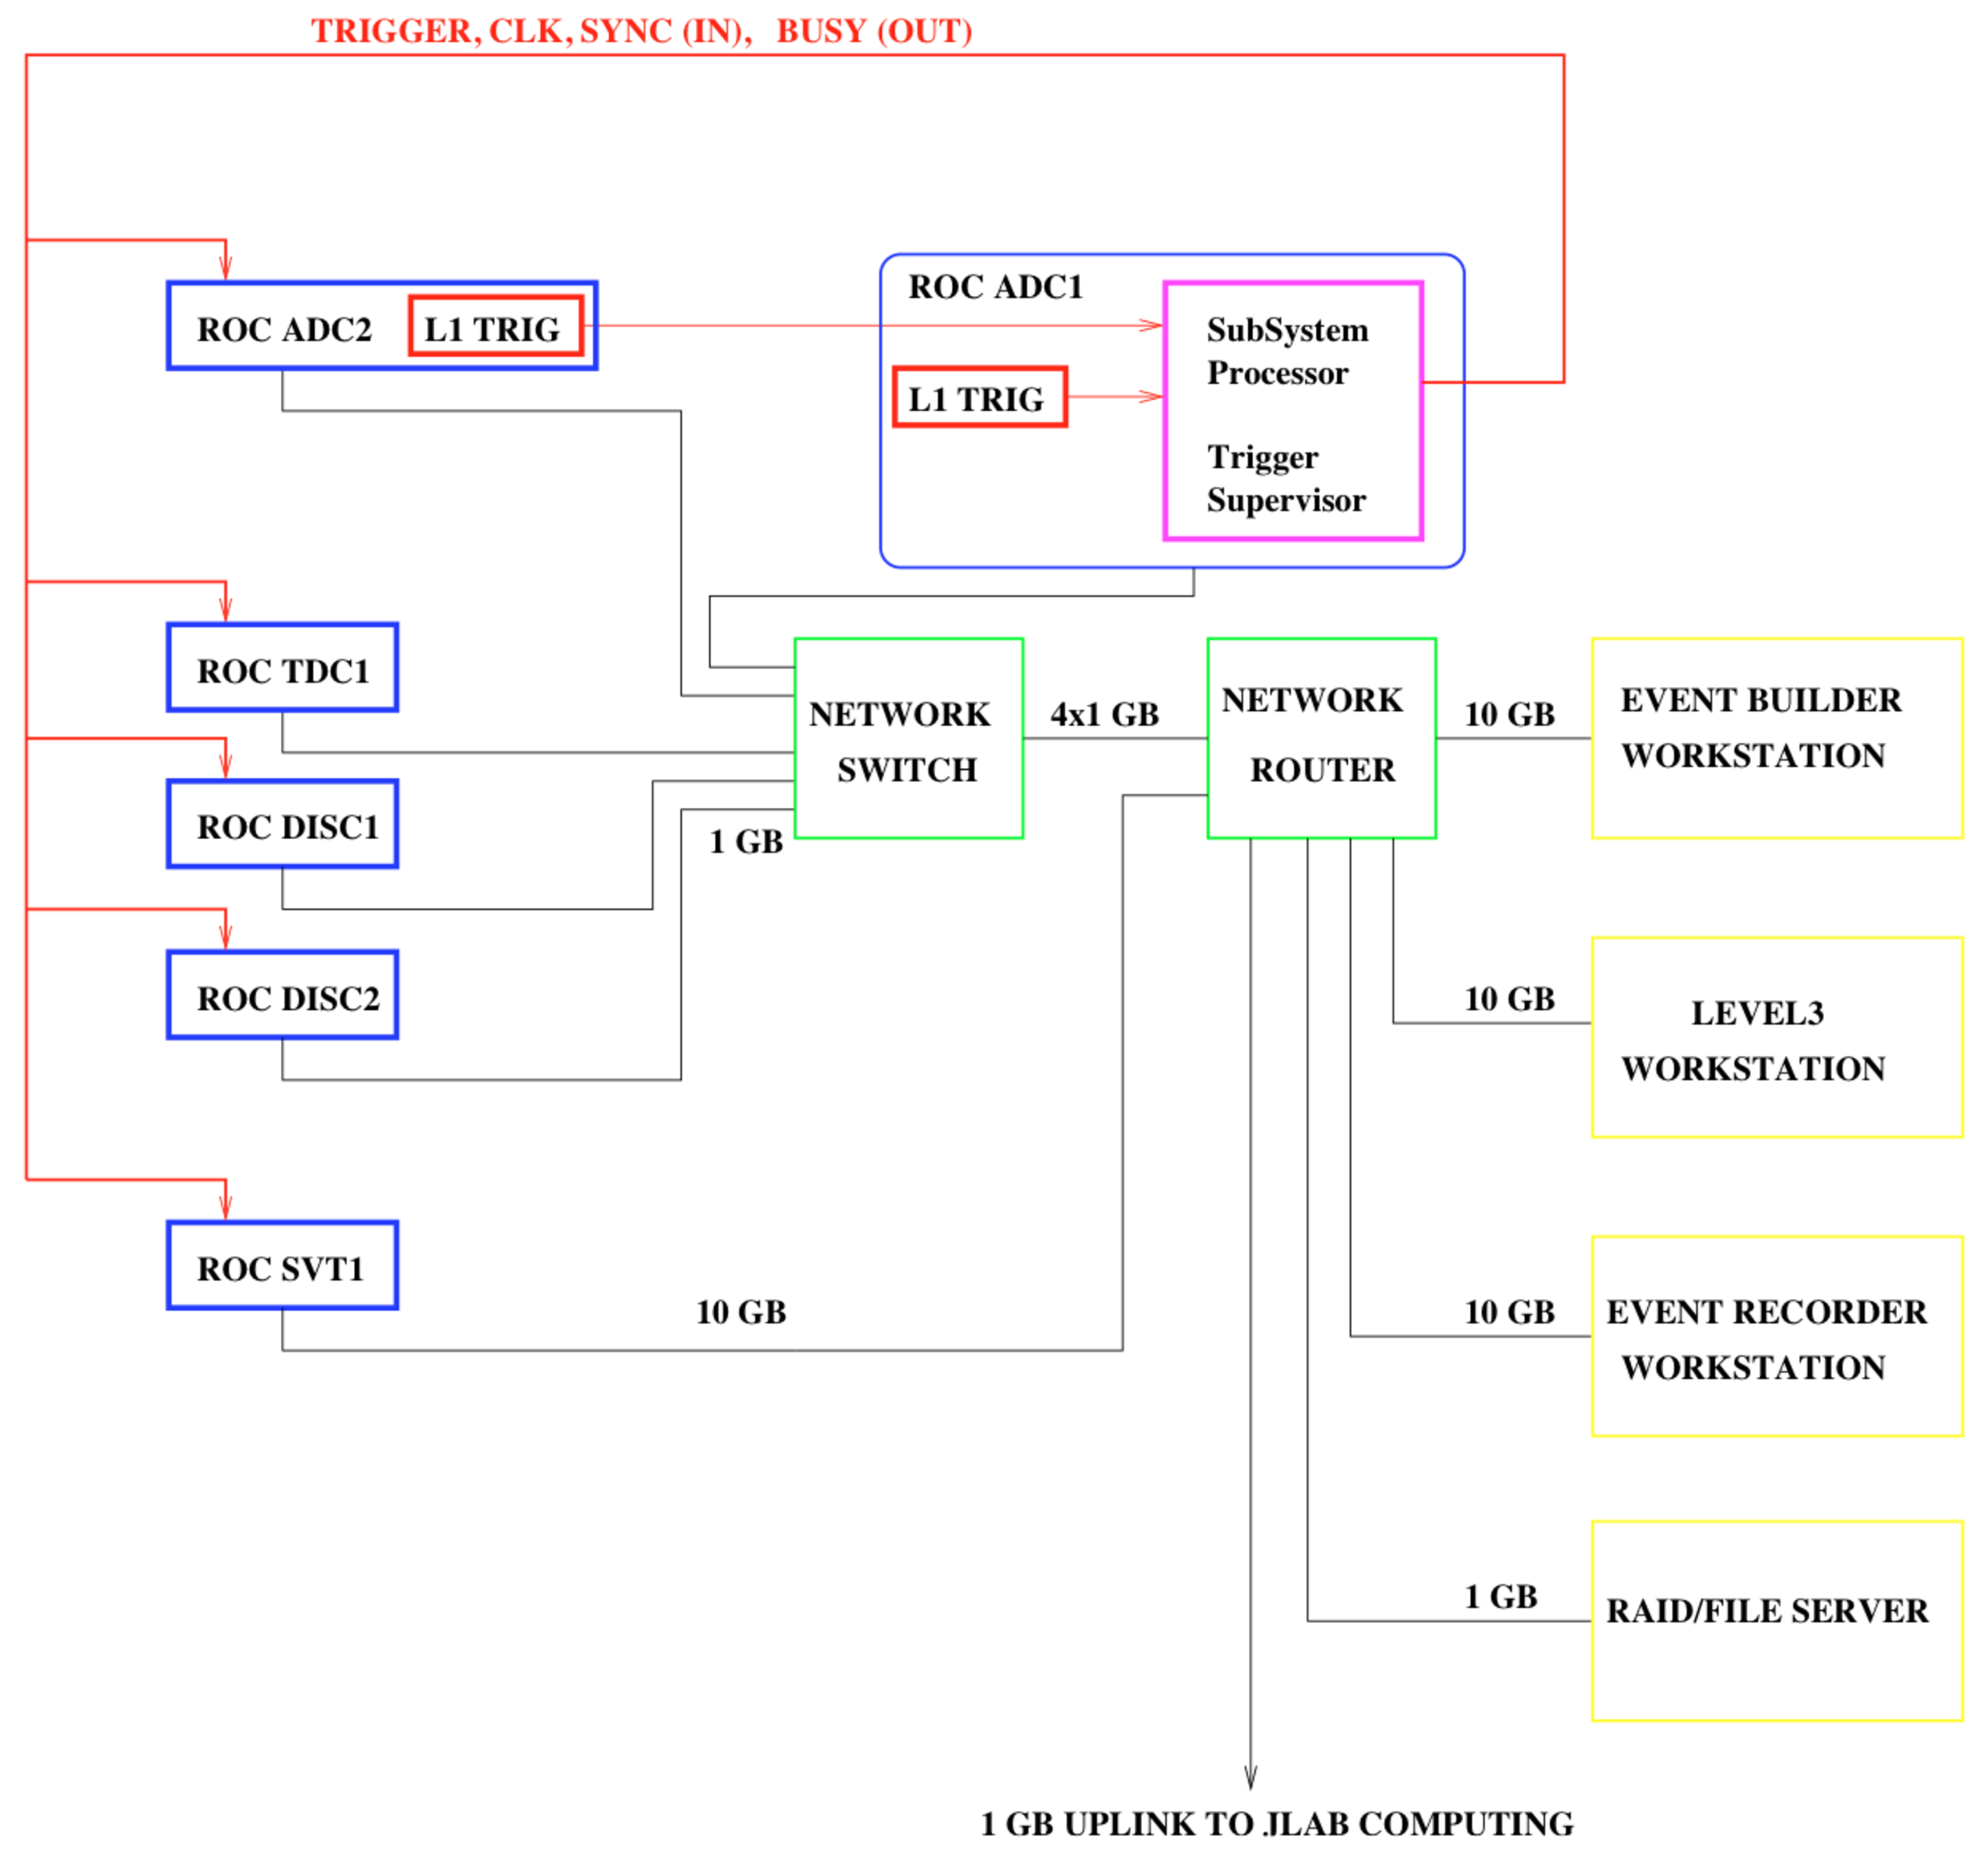
\includegraphics[ scale=0.3]{daq/figures/daq_schem.pdf}
\caption{\small{Schematic block diagram of the data acquisition system.}}
\label{fig:daq_hardware_overview}
\end{figure*}
The main software component is the Readout Controllers (ROCs) that collects information 
from the front end electronics board, processes it and sends to through the network to the 
Event Builder server. ROCs are installed in every crate holding front end boards. The 
VME based crates runs ROCs on mvme6100 controller boards with prpmc880 or pmc280 
coprocessor modules. {\color{red} Might need update?} The ROC for the SVT runs on 
a processor blade in the ATCA crate which handles the SVT part of the DAQ system. 
The Event Builder assembles 
information from the SVT, ECal and muon detector ROCs and assembles it into a single 
event which is passed to the (RAID5) data storage system capable of handling up to 
100MBytes/s. The Event Builder and other 
critical components run on multicore Opteron-based multi-CPU servers which is a 
sufficient configuration to handle HPS. The backbone of the DAQ network system is a 
Foundry router providing 1Gbit and 10Gbit connections between DAQ components and 
the JLab computing facility. The SVT ROC has a 10Gbit link to the Foundry router while the 
ROCs for the ECal and muon detector connect through a 1Gbit network switch. The long 
term data storage is handled by a 1Gbit uplink to the JLab computing facility. 

Section~\ref{sec:svt_daq} describes the SVT DAQ in more detail. The VXS based readout for 
the ECal and muon detector is described in Sec.~\ref{sec:fadc_daq} and the trigger 
system is explained in more detail in Sec.~\ref{sec:triggerdaq}.

\subsubsection{SVT Data Acquisition}
\label{sec:svt_daq}
The goal of the SVT DAQ is to support the continuous 40MHz readout and processing of signals from 
the 24 silicon strip sensors of the SVT and select those events that were identified by the 
Level 1 trigger system for transfer to the JLab DAQ for further event processing at rates 
close to 50kHz. 
Due to the difficult environment of the SVT with extreme occupancy and pile-up from multiple bunches  the number of noise hits has to be low to keep total data rates under control and 
each pulse from an energy deposition in the silicon needs to be sampled in order to facilitate 
reconstruction of the hit time to high accuracy. 

To meet these demanding requirements each of the 24 silicon strip sensors is connected to a 
hybrid board housing five 128-channel APV25~{\color{red}Reference needed} integrated circuits. The APV25, initially developed for the Compact Muon Solenoid silicon
 tracker~{\color{red}Reference needed}  at the Large Hadron Collider at CERN, was 
 chosen based on their good match to the HPS requirements. They provide amplification, 
 pipelining, and analog storage for trigger accepted events. For each 640-channel hybrid 
 board (shown in Fig.~\ref{fig:hybrid_and_apv25_testrun}
 \begin{figure*}[t]
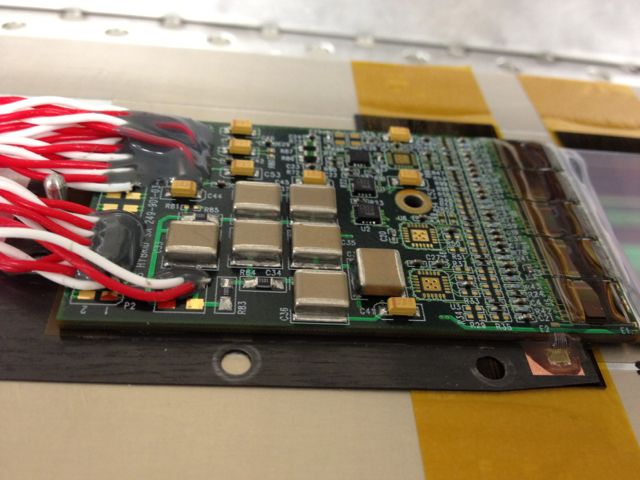
\includegraphics[ scale=0.3]{daq/figures/hybrid.jpg}
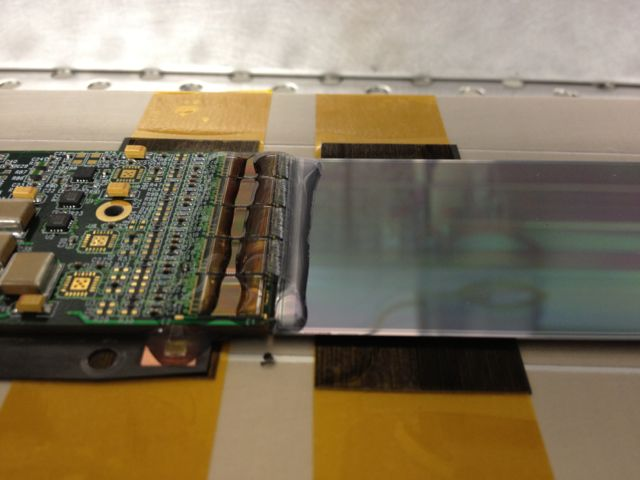
\includegraphics[ scale=0.3]{daq/figures/apvs-on-hybrid.jpg}
\caption{\small{Picture of a hybrid board from the test run in 2012 holding five 
APV25 ASICs that are wire bonded to the silicon sensor.}}
\label{fig:hybrid_and_apv25_testrun}
\end{figure*}
Each hybrid board has five analog output lines where analog data from each APV25 are 
sent using low power LVDS signals over about 3~m of multi-twisted-pair cable to a readout 
board. 

Figure~\ref{fig:svt_daq_overview} gives an overview of the SVT readout system. 
 \begin{figure*}[t]
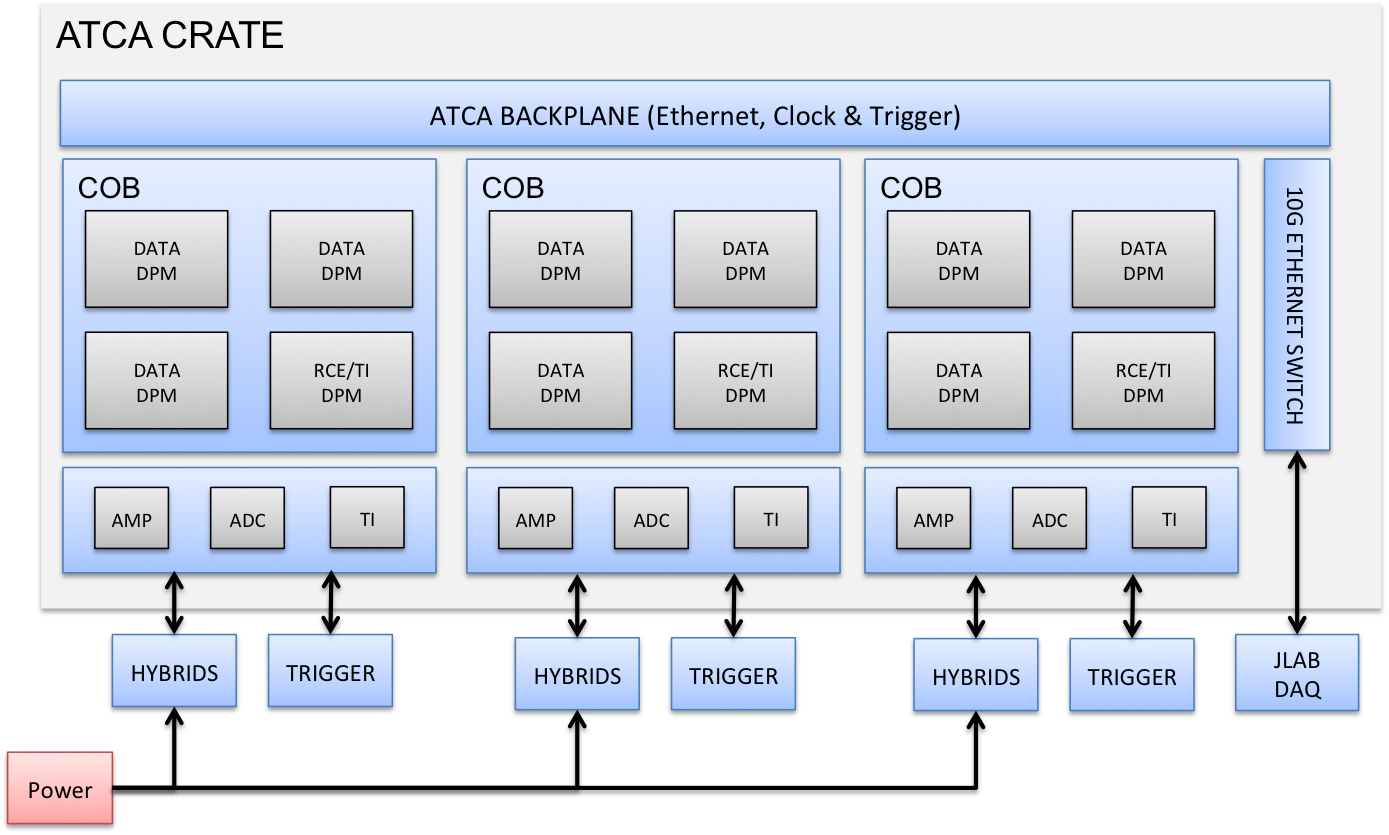
\includegraphics[ scale=0.6]{daq/figures/svt_daq_schem.png}
\caption{\small{Schematic block diagram of the SVT data acquisition system.}}
\label{fig:svt_daq_overview}
\end{figure*}
It is developed and built at SLAC using the Advanced Telecom 
Communication Architecture (ATCA) system for high speed data transfer. The analog signals 
from the 15,360 channels are digitized on the Rear Transition Module (RTM) boards. A 
pre-amplifier scales the APV25 differential current output to match the range of a 14-bit 
Analog to Digital Converter (ADC). Each RTM board has three sections that each service 
three hybrids. The ADC operates at the system clock frequency of 41.667~MHz. The RTM 
also has a 4-channel fiber optic module to communicate with the JLab trigger supervisor. 
A picture of a RTM board is shown in Fig.~\ref{fig:rtm_testrun}.
 \begin{figure*}[t]
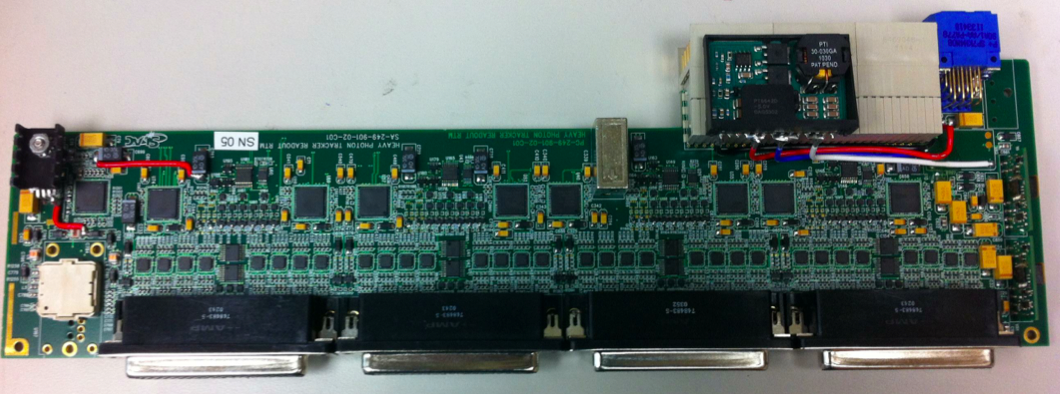
\includegraphics[ scale=0.25]{daq/figures/rtm.png}
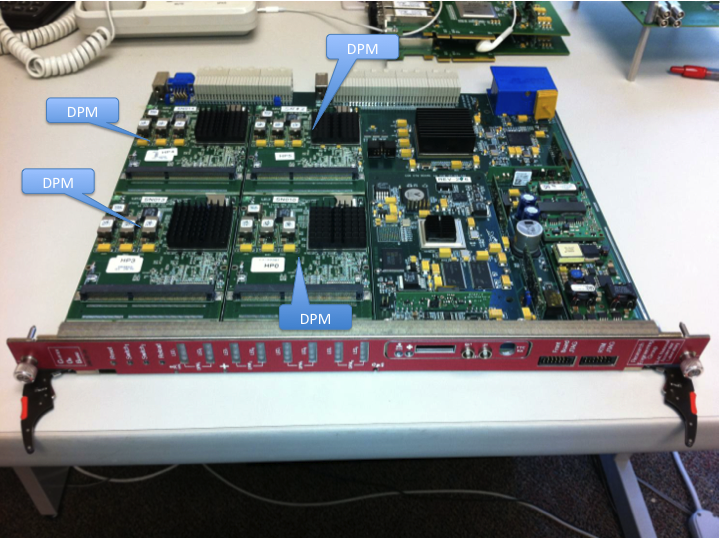
\includegraphics[ scale=0.4]{daq/figures/svt_daq_module_noted.png}
\caption{\small{Picture of a RTM (top) and COB board (bottom) 
used in the HPS test run 2012.}}
\label{fig:rtm_testrun}
\end{figure*}
The main COB board has four FPGA units that each interfaces with a single section of the 
the RTM.  Each FPGA is housed on a separate daughter board called 
Data Processing Module (DPM). Each DPM receives the digitized signals from the hybrids 
from the RTM, applies thresholds for data reduction and organizes the sample data 
into UDP datagrams. Each DPM also includes an I2C controller to configure and monitor the 
APV25 chips. One of the DPMs functions as the trigger interface which receives trigger 
signals from the optical fiber module on the RTM, handles distribution of clock and trigger 
and handles communication with the JLab trigger supervisor and the RCE. The 
RCE (Reconfigurable Cluster Element) is a generic computational building block 
on the trigger interface DPM running a 450~MHz PPC processor with 4GB of DDR3 
memory. Four COBs housed in a two ATCA crates is sufficient to handle 
the 36 hybrids of the SVT.

The RCE receives and buffers UDP datagrams from the data and trigger DPMs and
 assembles them into full event frames. The RCE also runs an implementation of the JLab ROC application that handles the integration of the SVT event frames into the JLab DAQ 
 system described above. The RCE node transfer data to the JLab DAQ  
 thorough a 10~Gbit Ethernet backend interface. 


The maximum readout rate of the SVT DAQ  is limited by the readout time 
of the APV25 chip. Using overlapping trigger and readout functionality, where the 
APV25 chip can buffer up to 5 triggers, the maximum average readout rate expected for 
HPS is 45kHz {\color{red} need verification}.   







\subsubsection{ECal and Muon Detector FADC Readout}
\label{sec:ecal_daq}
The main part of the readout of the ECal and muon detector are identical. Signals from each 
readout unit are sent to a signal splitter. For the ECal the charge signal from the APDs are 
shaped and amplified as described in Sec.~\ref{sec:ecal_readout} before feed into the 
splitter. One of the outputs of every splitter (for both the ECal and muon detector channels) 
feeds a separate channel on Flash ADC (FADC) readout boards that are packaged in 
16-channel VXS modules. Two VXS modules are used to accommodate the two ECal 
halves, each one with 221 channels, and a single VXS module is used to readout the muon 
detector. 

The FADCs stores the 12-but digitized samples of each channel in 8~$\mu$s deep pipelines. 
After a trigger is received a part of the pipeline corresponding to X number of samples 
before and Y samples after the signal passed a predefined threshold. Transferring only 
the time it passed threshold and a channel sum as energy estimate greatly reduces the data rate. 


The FADCs are an integral part of the HPS calorimeter trigger system. The output of each 
FADC channel in the same VXS module is collected by a crate trigger processor which performs cluster finding. The result from each create trigger processor (i.e. each half of 
the ECal) is combined in the sub-system processor module which applies further selections 
based on single- and combination of clusters to form a trigger decision passed to the trigger 
supervisor. The trigger process channel sum runs at 4~ns allowing to HPS to reach a 8~ns 
time resolution of the trigger time. This is an important part of improving 
the pattern recognition to reduce confusion in the tracker which has considerable longer 
integration times. 


See Sec.~\ref{sec:triggerdaq} for more details on the operation of the trigger system.


\subsubsection{Trigger System}
\label{sec:triggerdaq}


\subsubsection{Event Size and Data Rates}
The extreme radiation environment with tails of scattered beam imposing high occupancy
 puts strict requirements on high readout speed but consequently low noise readout to limit 
 the data rates. The event sizes and rates are based on estimates from detailed simulations 
 verified by measurements in the test run. 
  
As suggested in Sec.~\ref{sec:svt_desc}, the SVT will be operating at an effective threshold of three
times the noise level or an equivalent of 0.135\% occupancy. This translates to on average of 21 channels above threshold. Background studies (see Sec.~\ref{sec:hps_perf}) show that 
there are on average 10 tracks per event at a beam energy of 2.2~GeV and current of 
200~nA. With each track 
having on average 2 strips above threshold for each sensor there are on average 160 channels above threshold. Each of these channels will result in six digitized samples of the 
pulse shape giving in total of 1084 samples per event for the SVT.
Each channel has, in addition to the digitized samples,  header information that identifies the 
the channel number and it's chip address. The complete SVT event size also 
include the overhead from each FPGA and the JLab data stream bank header.  
With the average occupancy 
estimated above the expected event size is 3.6~kbytes corresponding to a data rate of 
approximately 155~Mbytes/s assuming an average trigger rate of 43~kHz.  
This high data rate is handled utilizing 
the 10~Gbit ethernet connections internally of the ATCA crate and also to the JLab DAQ.
{\color{red} (need to update these with the exact simulation of environment}


The data rate from the ECal and muon system is estimated from the same running 
conditions as the SVT above. Each each calorimeter or muon hit consist of 4 bytes 
with an 8 byte header for each FADC board. 
The main limitation is of the order of 50Mbytes/s from each VXS crate. For a 
10\% occupancy estimated in Sec.~\ref{sec:trig_rate} the ECal event size is approximately 0.4~kbytes which translates to a total data rate of approximately 18.9~Mbytes/s 
(split between the two VXS crates) well within the DAQ system design. 

The contribution from the muon system is small due to it's significantly lower number of channels. The system is readout by nine FADC boards in a single VXS crate. The event 
size for a 10\% occupancy level is 0.1~kbytes which translates to a data rate of 6~Mbytes/s. 

Table~\ref{tab:data_rates} summarizes the event size and data rates for the different 
sub-systems. 
\begin{table}[]
\centering
\begin{tabular}{l|c|c|c}
Sub-system & Occupancy(\%) & Event size (kB) & Data Rate (MB/s) \\
\hline
SVT & 0.135 & 4.5 & 203 \\
ECal & 10 & 0.4 & 19 \\
Muon & 10 & 0.1 & 6 \\
\hline
Total & - & 4.2 & 179 \\
\hline
\end{tabular}
\caption{{\small Occupancy, event size and data rate expected for beam energy of 2.2~GeV and a current of 200nA.} {\color{red}Need update}}
\label{tab:data_rates}
\end{table}
The dominant contribution comes from the SVT where irreducible real hits from the high occupancy is dominating the rates. Using high-speed data links it's still within the DAQ system and high performance RAID file servers it's within the the system design. 

The total data volume for a 2 week long production run is expected to be around 83Tb 
assuming a duty factor of 30\%.  For a longer run a Level~3 fast track trigger can 
be deployed to lower the data rates and total volume to be written to disk. 
